
%%%%%%%%%%%%%%%%%%%%%%%%%%%%%%%%%%%%%%%%%%%%%%%%%%%%%%%%%%%%%%%%%%%%%%%%%%%%%%%%%%%%%%%%
%% TEMPLATE
%%%%%%%%%%%%%%%%%%%%%%%%%%%%%%%%%%%%%%%%%%%%%%%%%%%%%%%%%%%%%%%%%%%%%%%%%%%%%%%%%%%%%%%%
% \rowcolor{lightgray!50}


% \begin{table}
% \scriptsize % 6pt
% \begin{center}
% \begin{tabular}{|l|l|l|l|l|l|l|l|l|}
% \hline
% Offline Augmentation            & P0F0R1   &          & P0F1R0   &          & P0F1R1   &          & P1F0R0   &           \\
% \hline
%                                 & mean     & std      & mean     & std      & mean     & std      & mean     & std       \\
% \hline
% mAP@0.5:0.75:0.05               & 87.140\% & 0.432\%  & 84.415\% & 3.471\%  & 91.113\% & 0.313\% & 79.403\% & 2.083\%    \\
% diode left                      & 92.234\% & 1.321\%  & 91.294\% & 11.021\% & 90.803\% & 2.624\% & 85.666\% & 6.769\%    \\
% diode top                       & 94.578\% & 5.028\%  & 97.637\% & 2.344\%  & 97.840\% & 1.975\% & 93.787\% & 1.538\%    \\
% diode right                     & 91.243\% & 1.669\%  & 93.301\% & 4.324\%  & 94.277\% & 0.624\% & 94.306\% & 1.645\%    \\
% diode bottom                    & 90.823\% & 1.872\%  & 84.067\% & 10.039\% & 95.018\% & 3.899\% & 73.765\% & 16.099\%   \\
% resistor horizontal             & 97.046\% & 3.405\%  & 94.047\% & 4.202\%  & 98.570\% & 1.540\% & 84.394\% & 1.470\%    \\
% resistor vertical               & 95.147\% & 5.910\%  & 95.420\% & 3.709\%  & 96.094\% & 4.142\% & 90.873\% & 6.573\%    \\
% capacitor horizontal            & 93.635\% & 2.761\%  & 96.318\% & 1.487\%  & 97.084\% & 1.654\% & 94.134\% & 3.223\%    \\
% capacitor vertical              & 91.722\% & 6.025\%  & 91.730\% & 3.580\%  & 94.169\% & 2.593\% & 88.688\% & 2.366\%    \\
% ground left                     & 94.520\% & 2.395\%  & 89.788\% & 2.521\%  & 94.771\% & 1.759\% & 92.257\% & 0.852\%    \\
% ground top                      & 89.806\% & 4.827\%  & 83.703\% & 10.054\% & 89.804\% & 5.464\% & 79.250\% & 9.105\%    \\
% ground right                    & 87.742\% & 2.412\%  & 90.646\% & 6.170\%  & 94.216\% & 1.081\% & 82.389\% & 4.109\%    \\
% ground bottom                   & 90.629\% & 2.506\%  & 97.206\% & 1.084\%  & 96.884\% & 1.538\% & 91.053\% & 2.011\%    \\
% inductor horizontal             & 97.763\% & 2.858\%  & 86.493\% & 9.296\%  & 97.326\% & 2.945\% & 85.473\% & 2.084\%    \\
% inductor vertical               & 93.382\% & 3.552\%  & 90.954\% & 4.338\%  & 96.304\% & 2.290\% & 92.229\% & 6.615\%    \\
% source horizontal               & 95.718\% & 5.079\%  & 91.954\% & 4.404\%  & 97.915\% & 1.475\% & 90.277\% & 0.305\%    \\
% source vertical                 & 98.336\% & 0.313\%  & 96.963\% & 1.952\%  & 98.584\% & 0.396\% & 87.670\% & 6.401\%    \\
% current horizontal              & 95.852\% & 2.444\%  & 96.302\% & 2.777\%  & 98.804\% & 0.470\% & 92.569\% & 1.106\%    \\
% current vertical                & 97.209\% & 2.439\%  & 94.627\% & 2.585\%  & 97.680\% & 2.010\% & 93.514\% & 5.561\%    \\
% text                            & 69.993\% & 1.410\%  & 71.140\% & 5.502\%  & 77.819\% & 3.669\% & 67.715\% & 2.369\%    \\
% arrow left                      & 42.737\% & 1.960\%  & 33.867\% & 2.496\%  & 57.432\% & 5.763\% & 24.293\% & 3.328\%    \\
% arrow top                       & 75.880\% & 7.437\%  & 56.755\% & 11.619\% & 83.454\% & 1.074\% & 40.397\% & 8.439\%    \\
% arrow right                     & 59.931\% & 14.305\% & 55.652\% & 5.557\%  & 70.008\% & 9.051\% & 45.171\% & 7.226\%    \\
% arrow bottom                    & 68.291\% & 3.777\%  & 61.672\% & 3.133\%  & 80.737\% & 5.176\% & 56.408\% & 11.852\%   \\
% \hline
% \\\\\\
% \hline
% Offline Augmentation            & P1F0R1   &          & P1F1R0   &          & 1F1R1    &           & Baseline &          \\
% \hline
%                                 & mean     & std      & mean     & std      & mean     & std       & mean     & std      \\
% \hline
% mAP@0.5:0.75:0.05               & 89.641\% & 0.106\%  & 86.129\% & 0.229\%  &  92.578\%  & 0.409\% & 73.415\% & 0.846\%  \\
% diode left                      & 93.597\% & 4.014\%  & 91.181\% & 7.667\%  &  92.333\%  & 4.550\% & 75.587\% & 16.873\% \\
% diode top                       & 91.681\% & 1.473\%  & 97.798\% & 2.010\%  &  96.948\%  & 1.737\% & 87.505\% & 10.368\% \\
% diode right                     & 91.757\% & 3.252\%  & 89.021\% & 4.762\%  &  93.518\%  & 4.222\% & 87.168\% & 3.649\%  \\
% diode bottom                    & 94.280\% & 4.056\%  & 81.750\% & 2.703\%  &  95.016\%  & 3.342\% & 79.644\% & 4.437\%  \\
% resistor horizontal             & 95.806\% & 3.506\%  & 93.281\% & 3.849\%  &  97.322\%  & 0.526\% & 75.920\% & 7.097\%  \\
% resistor vertical               & 97.179\% & 1.734\%  & 99.284\% & 0.649\%  &  97.359\%  & 1.835\% & 90.844\% & 2.174\%  \\
% capacitor horizontal            & 99.293\% & 0.670\%  & 97.800\% & 0.587\%  &  98.232\%  & 1.589\% & 87.420\% & 3.080\%  \\
% capacitor vertical              & 94.622\% & 1.469\%  & 87.713\% & 3.641\%  &  94.118\%  & 4.588\% & 78.861\% & 7.128\%  \\
% ground left                     & 96.220\% & 4.299\%  & 94.495\% & 3.422\%  &  96.770\%  & 1.317\% & 87.967\% & 9.064\%  \\
% ground top                      & 93.892\% & 2.475\%  & 83.231\% & 9.478\%  &  93.935\%  & 3.310\% & 63.528\% & 12.543\% \\
% ground right                    & 91.405\% & 2.666\%  & 83.262\% & 4.277\%  &  90.997\%  & 0.904\% & 78.510\% & 2.877\%  \\
% ground bottom                   & 98.080\% & 1.169\%  & 94.569\% & 5.678\%  &  98.260\%  & 1.757\% & 82.913\% & 2.825\%  \\
% inductor horizontal             & 97.153\% & 2.481\%  & 93.622\% & 0.712\%  &  99.342\%  & 0.585\% & 89.902\% & 7.664\%  \\
% inductor vertical               & 95.204\% & 3.354\%  & 93.947\% & 1.989\%  &  97.193\%  & 1.906\% & 80.216\% & 7.083\%  \\
% source horizontal               & 97.212\% & 1.229\%  & 94.548\% & 3.643\%  &  97.966\%  & 1.765\% & 91.016\% & 3.320\%  \\
% source vertical                 & 96.283\% & 1.995\%  & 94.320\% & 0.996\%  &  96.674\%  & 2.675\% & 92.630\% & 2.238\%  \\
% current horizontal              & 97.694\% & 2.175\%  & 97.485\% & 0.323\%  &  100.000\% & 0.000\% & 89.566\% & 4.880\%  \\
% current vertical                & 98.231\% & 1.539\%  & 94.763\% & 3.435\%  &  98.055\%  & 2.632\% & 90.530\% & 4.228\%  \\
% text                            & 77.341\% & 0.219\%  & 77.322\% & 1.650\%  &  83.885\%  & 1.505\% & 59.403\% & 1.547\%  \\
% arrow left                      & 54.932\% & 6.911\%  & 50.885\% & 0.934\%  &  65.458\%  & 5.535\% & 13.468\% & 11.740\% \\
% arrow top                       & 72.627\% & 2.817\%  & 63.662\% & 2.807\%  &  85.952\%  & 3.736\% & 24.602\% & 9.146\%  \\
% arrow right                     & 63.998\% & 3.719\%  & 54.102\% & 3.586\%  &  79.383\%  & 3.489\% & 44.401\% & 8.481\%  \\
% arrow bottom                    & 73.246\% & 6.320\%  & 72.935\% & 4.459\%  &  80.567\%  & 1.846\% & 36.938\% & 4.996\%  \\
% \hline

% \end{tabular}
% \caption{The results of the offline augmentation configuration search. The configuration should be interpreted in a way that a 1 behind a letter means that particular augmentation is enabled. Further, the letter ``P'' stands for projection, ``F'' for flip and ``R'' means rotation. Rotation always includes a 90\textdegree\, 180\textdegree\ and a 270\textdegree\ rotation. Flip is a horizontal flip. Additionally, when flip and rotation are enabled at the same time the flipped imaged gets also rotated three times. All results are again given with the mean and standard deviation over three runs and the results are compared against the baseline, which is the best performing learning rate from the learning rate search experiment (table \ref{tab:yolo_init_lr_results}).}
% \label{tab:yolo_offline_aug_results}
% \end{center}
% \end{table}

%%%%%%%%%%%%%%%%%%%%%%%%%%%%%%%%%%%%%%%%%%%%%%%%%%%%%%%%%%%%%%%%%%%%%%%%%%%%%%%%%%%%%%%%
%% TEMPLATE 2
%%%%%%%%%%%%%%%%%%%%%%%%%%%%%%%%%%%%%%%%%%%%%%%%%%%%%%%%%%%%%%%%%%%%%%%%%%%%%%%%%%%%%%%%
% \begin{table}
% \scriptsize % 6pt
% \begin{center}
% \begin{tabular}{|l|l|l|l|l|l|l|l|l|}
% \hline
% Rotation                        & 10\textdegree\   &   & 20\textdegree\ &     & 30\textdegree\ &     & Baseline &              \\
% \hline
%                                 & mean     & std      & mean     & std      & mean     & std      & mean     & std          \\
% \hline
% mAP@0.5:0.75:0.05               & 95.368\%  & 0.388\%  & 94.521\%  & 0.046\%  & 94.198\%  & 0.464\% & 92.578\%  & 0.409\%   \\
% diode left                      & 93.276\%  & 2.454\%  & 93.879\%  & 1.966\%  & 95.265\%  & 3.030\% & 92.333\%  & 4.550\%   \\
% diode top                       & 99.327\%  & 1.165\%  & 98.394\%  & 1.564\%  & 99.436\%  & 0.977\% & 96.948\%  & 1.737\%   \\
% diode right                     & 99.198\%  & 0.762\%  & 96.956\%  & 1.386\%  & 97.650\%  & 2.048\% & 93.518\%  & 4.222\%   \\
% diode bottom                    & 95.149\%  & 2.444\%  & 94.065\%  & 2.119\%  & 91.071\%  & 2.280\% & 95.016\%  & 3.342\%   \\
% resistor horizontal             & 100.000\% & 0.000\%  & 100.000\% & 0.000\%  & 98.245\%  & 0.775\% & 97.322\%  & 0.526\%   \\
% resistor vertical               & 97.537\%  & 2.241\%  & 97.330\%  & 2.359\%  & 98.698\%  & 2.255\% & 97.359\%  & 1.835\%   \\
% capacitor horizontal            & 97.545\%  & 1.114\%  & 97.043\%  & 0.570\%  & 96.277\%  & 3.629\% & 98.232\%  & 1.589\%   \\
% capacitor vertical              & 94.609\%  & 1.019\%  & 92.022\%  & 2.187\%  & 95.924\%  & 3.782\% & 94.118\%  & 4.588\%   \\
% ground left                     & 98.785\%  & 1.311\%  & 98.399\%  & 0.406\%  & 94.828\%  & 2.016\% & 96.770\%  & 1.317\%   \\
% ground top                      & 96.769\%  & 0.811\%  & 95.385\%  & 4.197\%  & 93.485\%  & 2.550\% & 93.935\%  & 3.310\%   \\
% ground right                    & 98.152\%  & 0.929\%  & 96.896\%  & 1.449\%  & 93.781\%  & 0.777\% & 90.997\%  & 0.904\%   \\
% ground bottom                   & 97.540\%  & 0.740\%  & 97.735\%  & 0.791\%  & 98.538\%  & 0.611\% & 98.260\%  & 1.757\%   \\
% inductor horizontal             & 99.449\%  & 0.955\%  & 98.613\%  & 1.814\%  & 99.441\%  & 0.968\% & 99.342\%  & 0.585\%   \\
% inductor vertical               & 96.846\%  & 1.177\%  & 95.766\%  & 2.795\%  & 97.990\%  & 1.334\% & 97.193\%  & 1.906\%   \\
% source horizontal               & 99.352\%  & 0.575\%  & 98.567\%  & 1.195\%  & 97.685\%  & 2.474\% & 97.966\%  & 1.765\%   \\
% source vertical                 & 99.188\%  & 0.273\%  & 98.998\%  & 1.289\%  & 98.932\%  & 1.302\% & 96.674\%  & 2.675\%   \\
% current horizontal              & 100.000\% & 0.000\%  & 100.000\% & 0.000\%  & 100.000\% & 0.000\% & 100.000\% & 0.000\%   \\
% current vertical                & 96.787\%  & 0.755\%  & 99.667\%  & 0.577\%  & 98.788\%  & 1.118\% & 98.055\%  & 2.632\%   \\
% text                            & 89.967\%  & 5.288\%  & 88.700\%  & 3.258\%  & 86.481\%  & 3.616\% & 83.885\%  & 1.505\%   \\
% arrow left                      & 86.635\%  & 10.788\% & 78.791\%  & 9.348\%  & 78.060\%  & 7.895\% & 65.458\%  & 5.535\%   \\
% arrow top                       & 90.350\%  & 3.327\%  & 89.965\%  & 1.384\%  & 91.907\%  & 3.234\% & 85.952\%  & 3.736\%   \\
% arrow right                     & 82.225\%  & 14.839\% & 81.451\%  & 10.183\% & 84.894\%  & 4.084\% & 79.383\%  & 3.489\%   \\
% arrow bottom                    & 84.769\%  & 3.433\%  & 85.361\%  & 6.232\%  & 79.179\%  & 5.651\% & 80.567\%  & 1.846\%   \\
% \hline

% \end{tabular}
% \caption{The results of the rotation augmentation, performed on different parameters and compared against the best offline augmentation configuration. Results with mean and standard deviation over three runs.}
% \label{tab:yolo_rotation_augmentation_result}
% \end{center}
% \end{table}


%%%%%%%%%%%%%%%%%%%%%%%%%%%%%%%%%%%%%%%%%%%%%%%%%%%%%%%%%%%%%%%%%%%%%%%%%%%%%%%%%%%%%%%%
%% APPENDIX BEGIN
%%%%%%%%%%%%%%%%%%%%%%%%%%%%%%%%%%%%%%%%%%%%%%%%%%%%%%%%%%%%%%%%%%%%%%%%%%%%%%%%%%%%%%%%
\clearpage
\section{MobileNetV2-UNet Experiments}
\label{app:munet_experiments}

\begin{figure}[H]
\begin{center}
    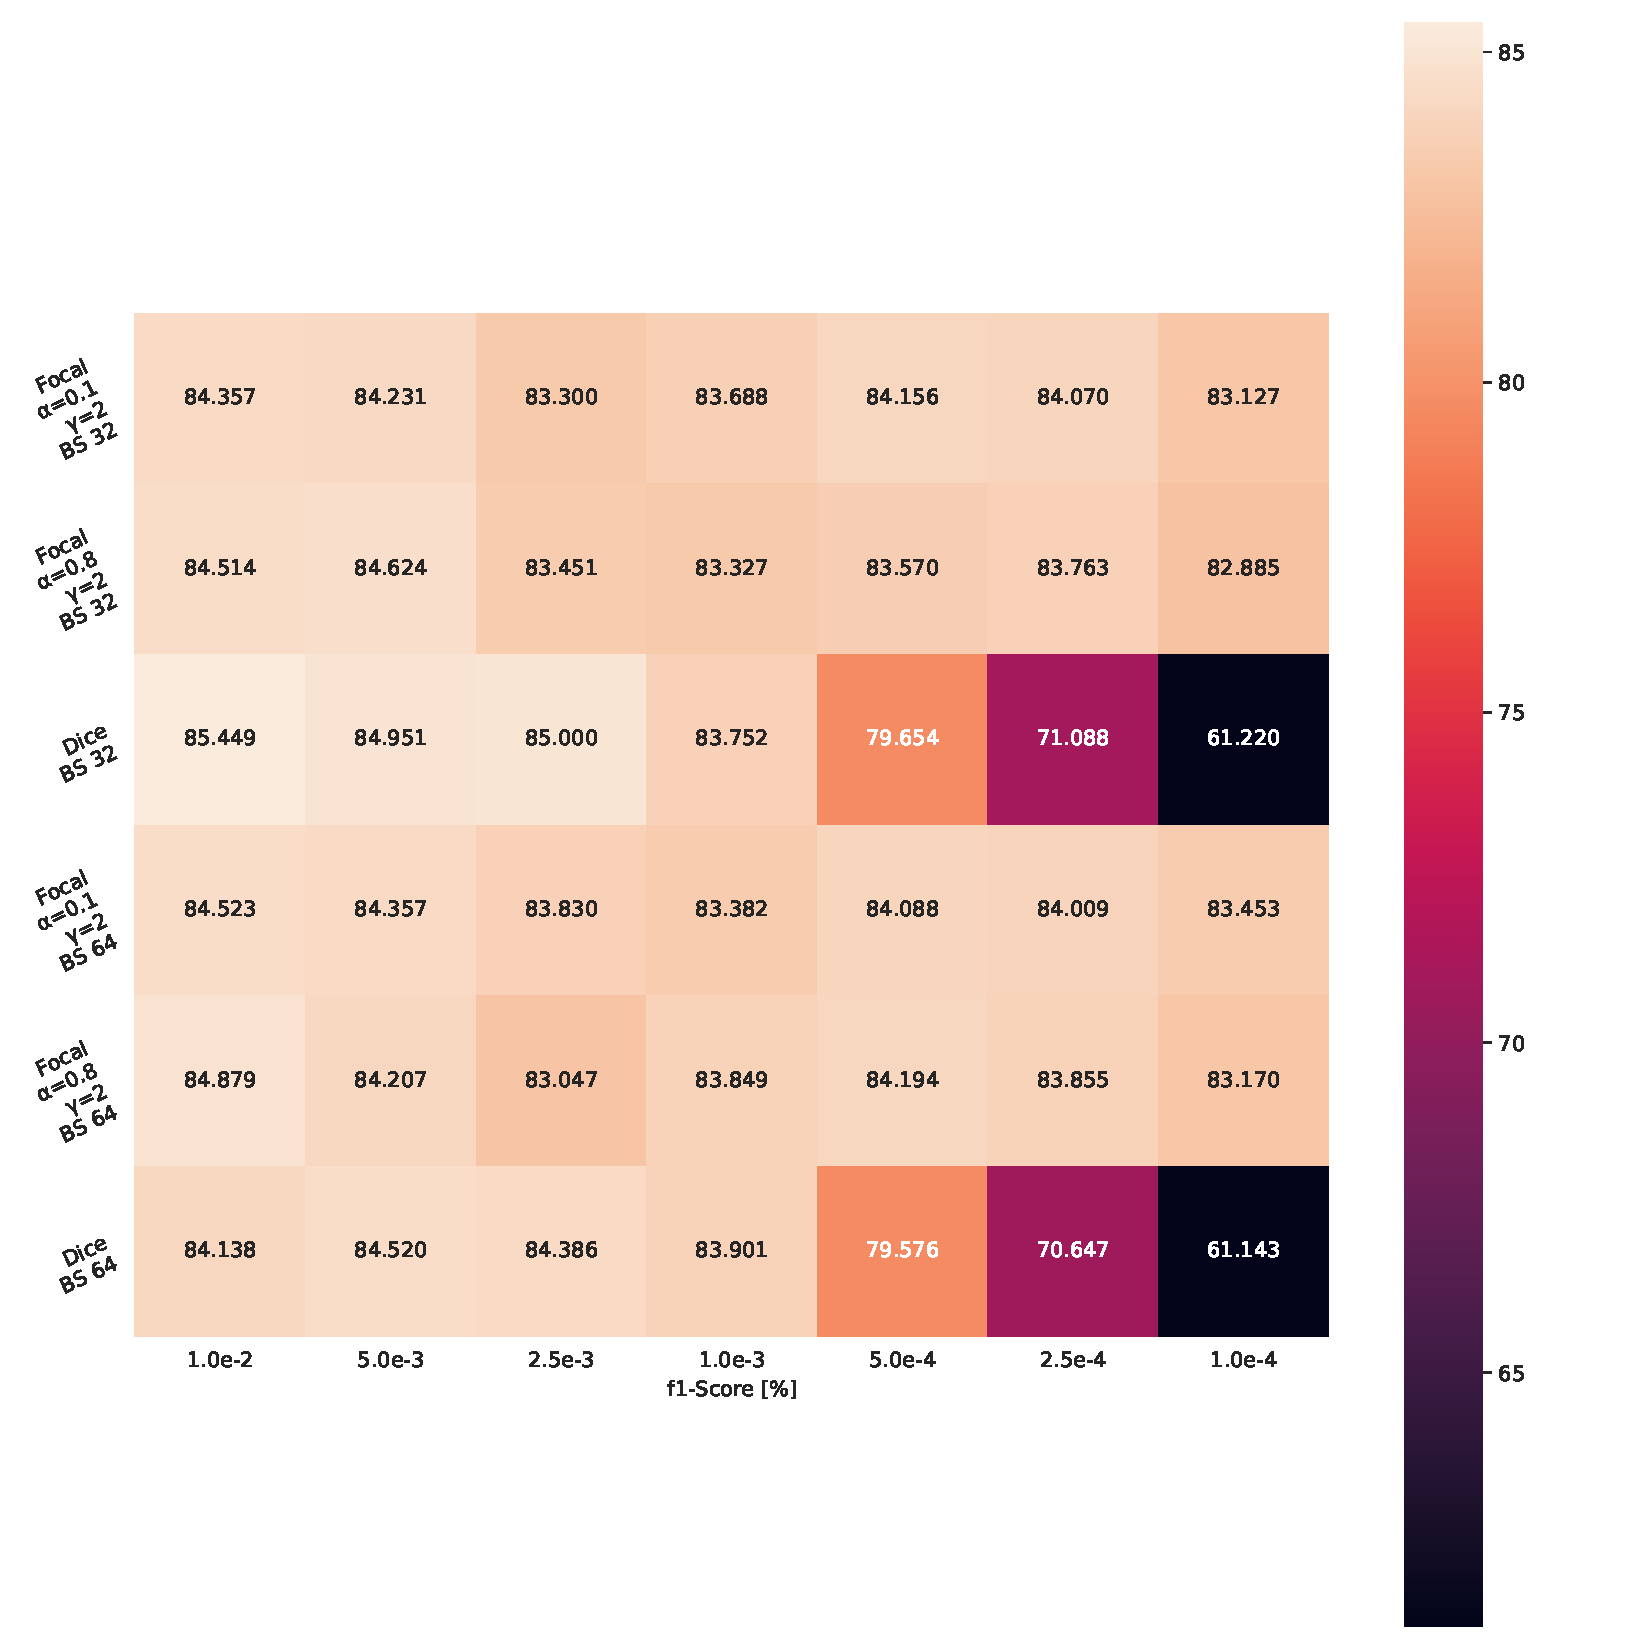
\includegraphics[width=\columnwidth]{imgs/munet_grid_heat_F1_B.pdf}
    \caption{F1-Score results of the \ac{MUnet} grid search experiment shown on the full validation data. Results are shown combined for the loss and batch size against the learning rate.}
    \label{fig:munet_f1b_heat}
\end{center}
\end{figure}

\begin{figure}[H]
\begin{center}
    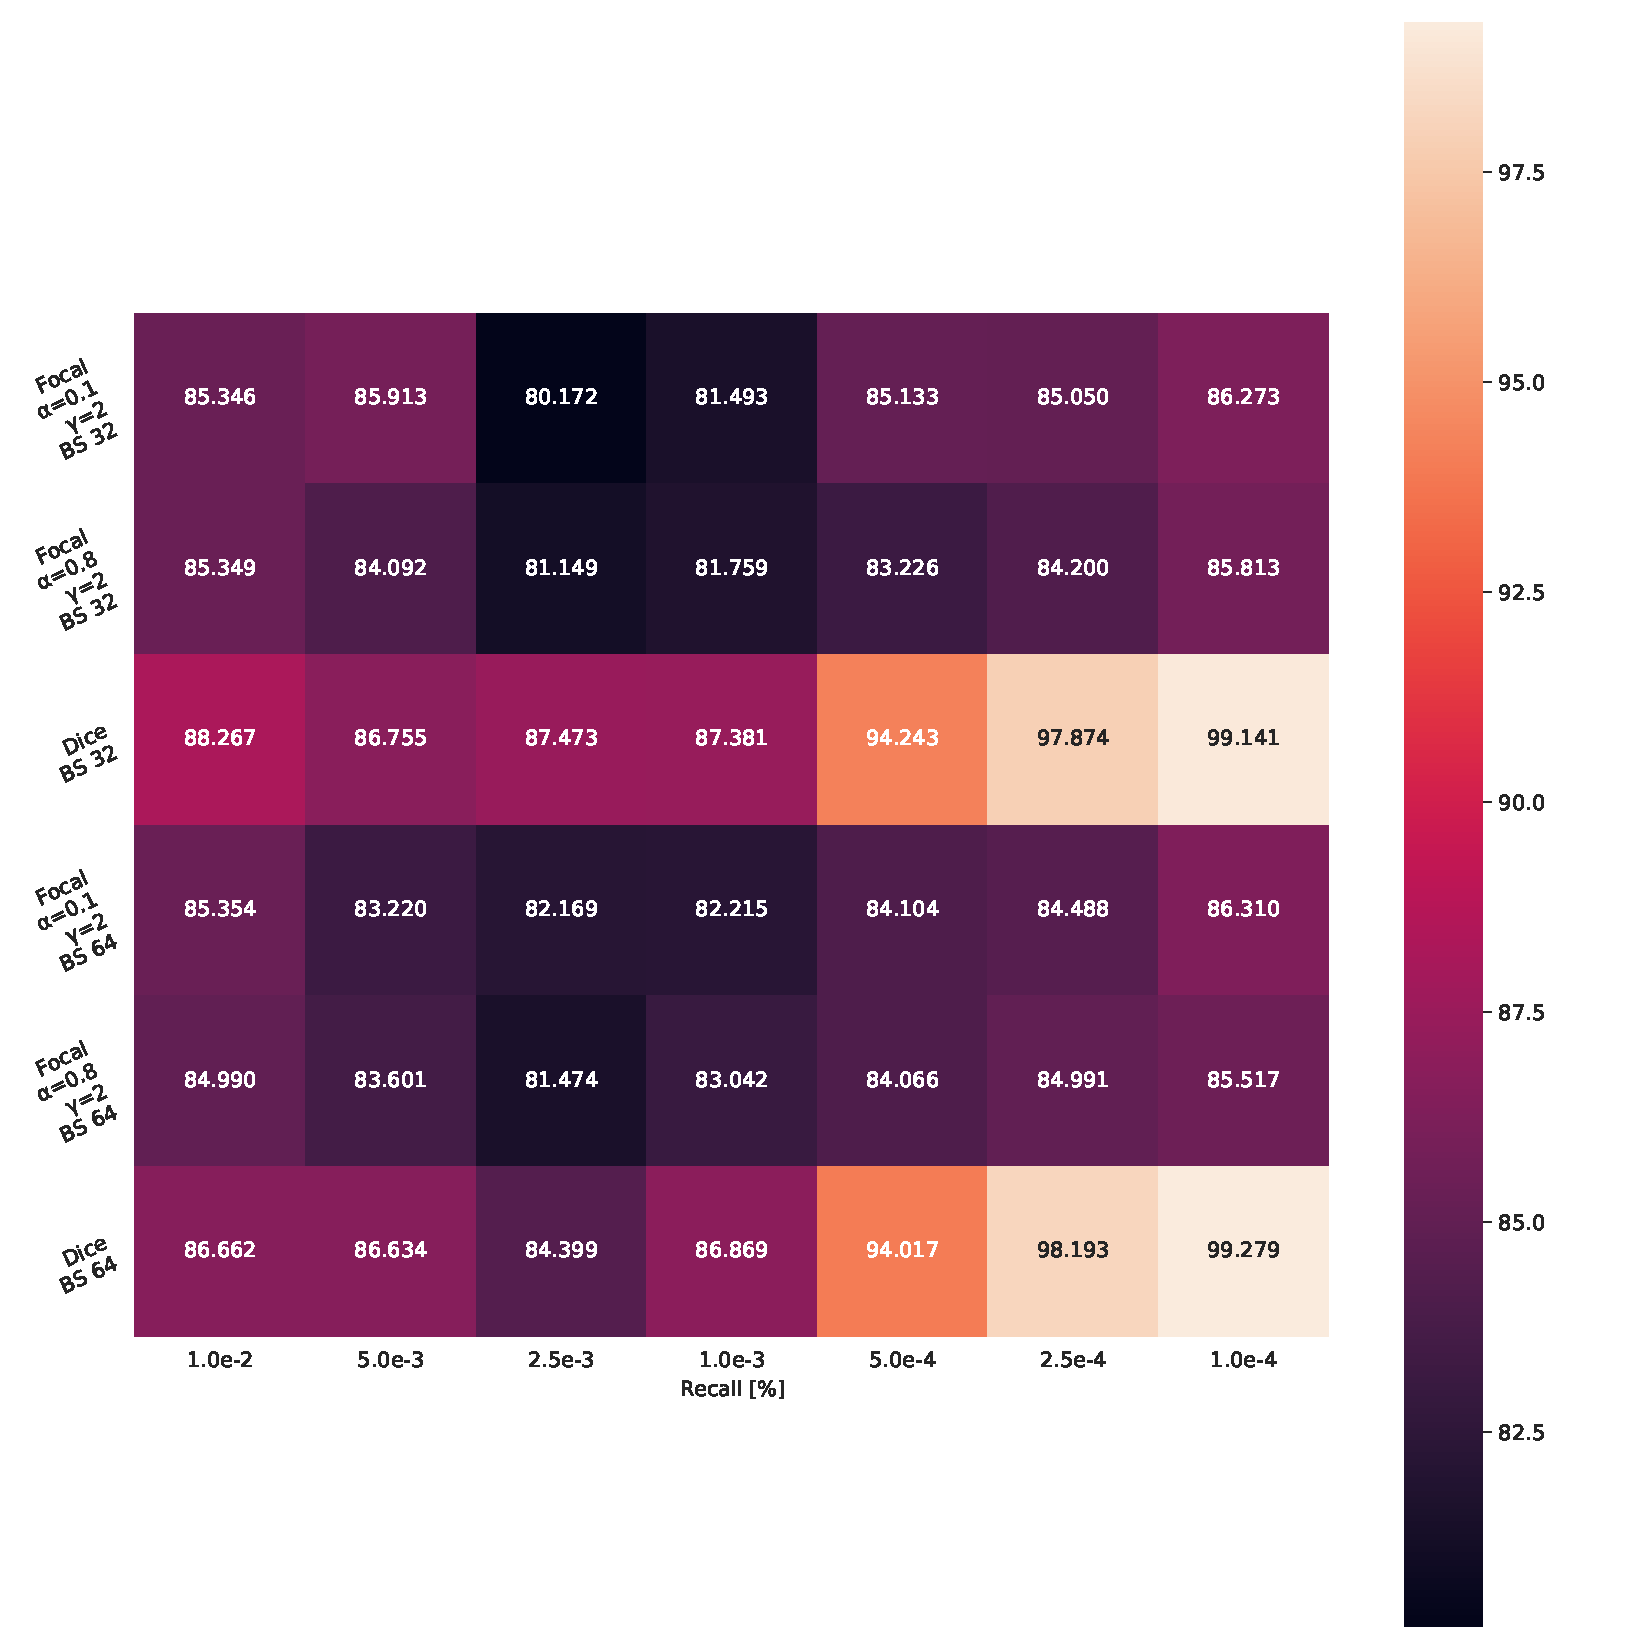
\includegraphics[width=\columnwidth]{imgs/munet_grid_heat_R_B.pdf}
    \caption{Recall results of the \ac{MUnet} grid search experiment shown on the full validation data. Results are shown combined for the loss and batch size against the learning rate.}
    \label{fig:munet_rb_heat}
\end{center}
\end{figure}

\begin{figure}[H]
\begin{center}
    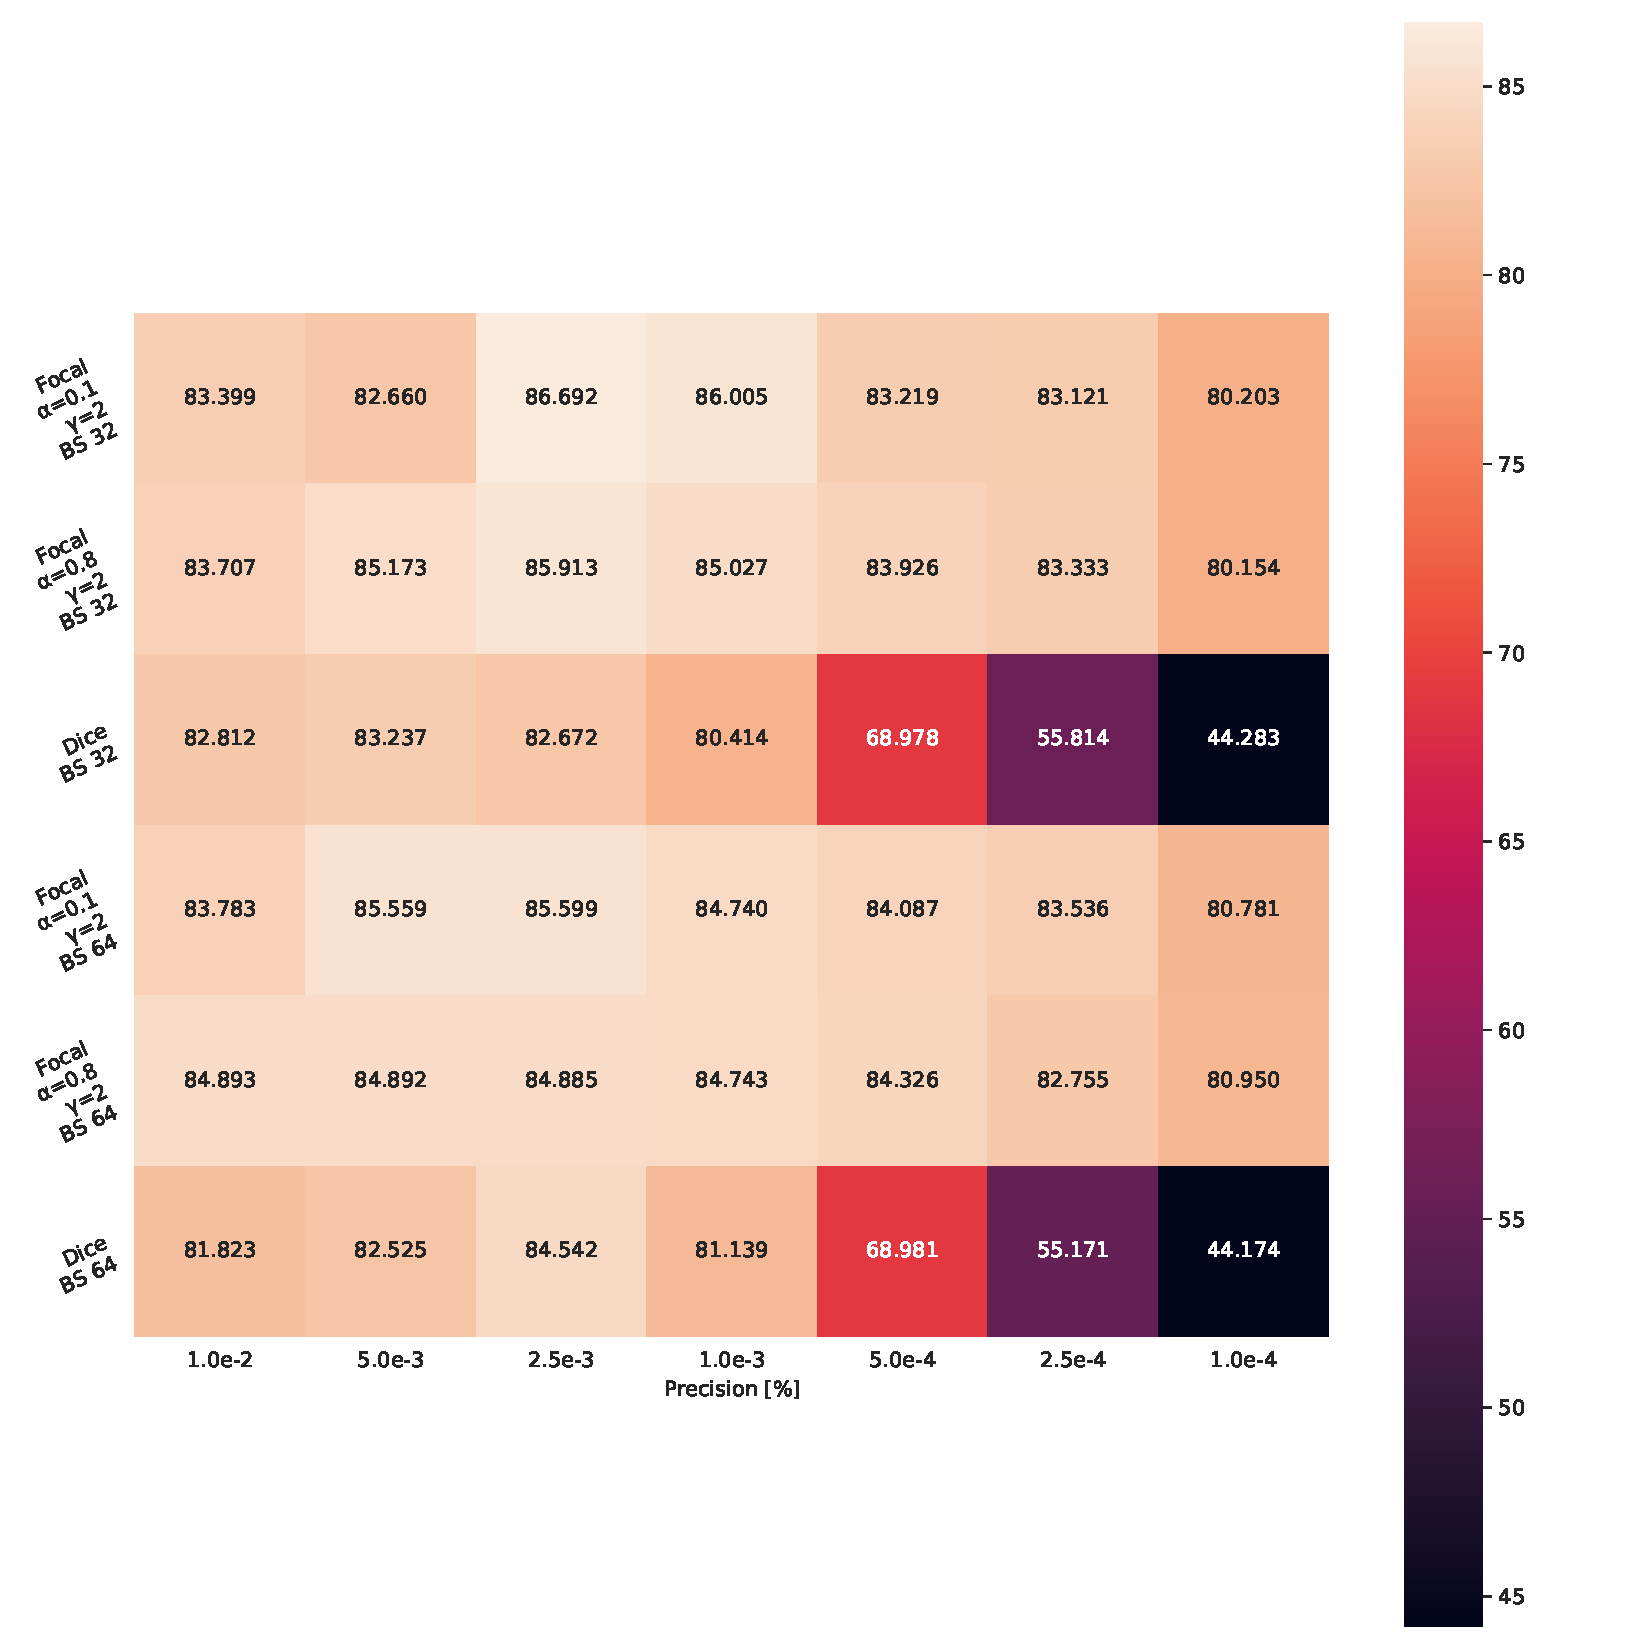
\includegraphics[width=\columnwidth]{imgs/munet_grid_heat_P_B.pdf}
    \caption{Precision results of the \ac{MUnet} grid search experiment shown on the full validation data. Results are shown combined for the loss and batch size against the learning rate.}
    \label{fig:munet_pb_heat}
\end{center}
\end{figure}

\begin{figure}[H]
\begin{center}
    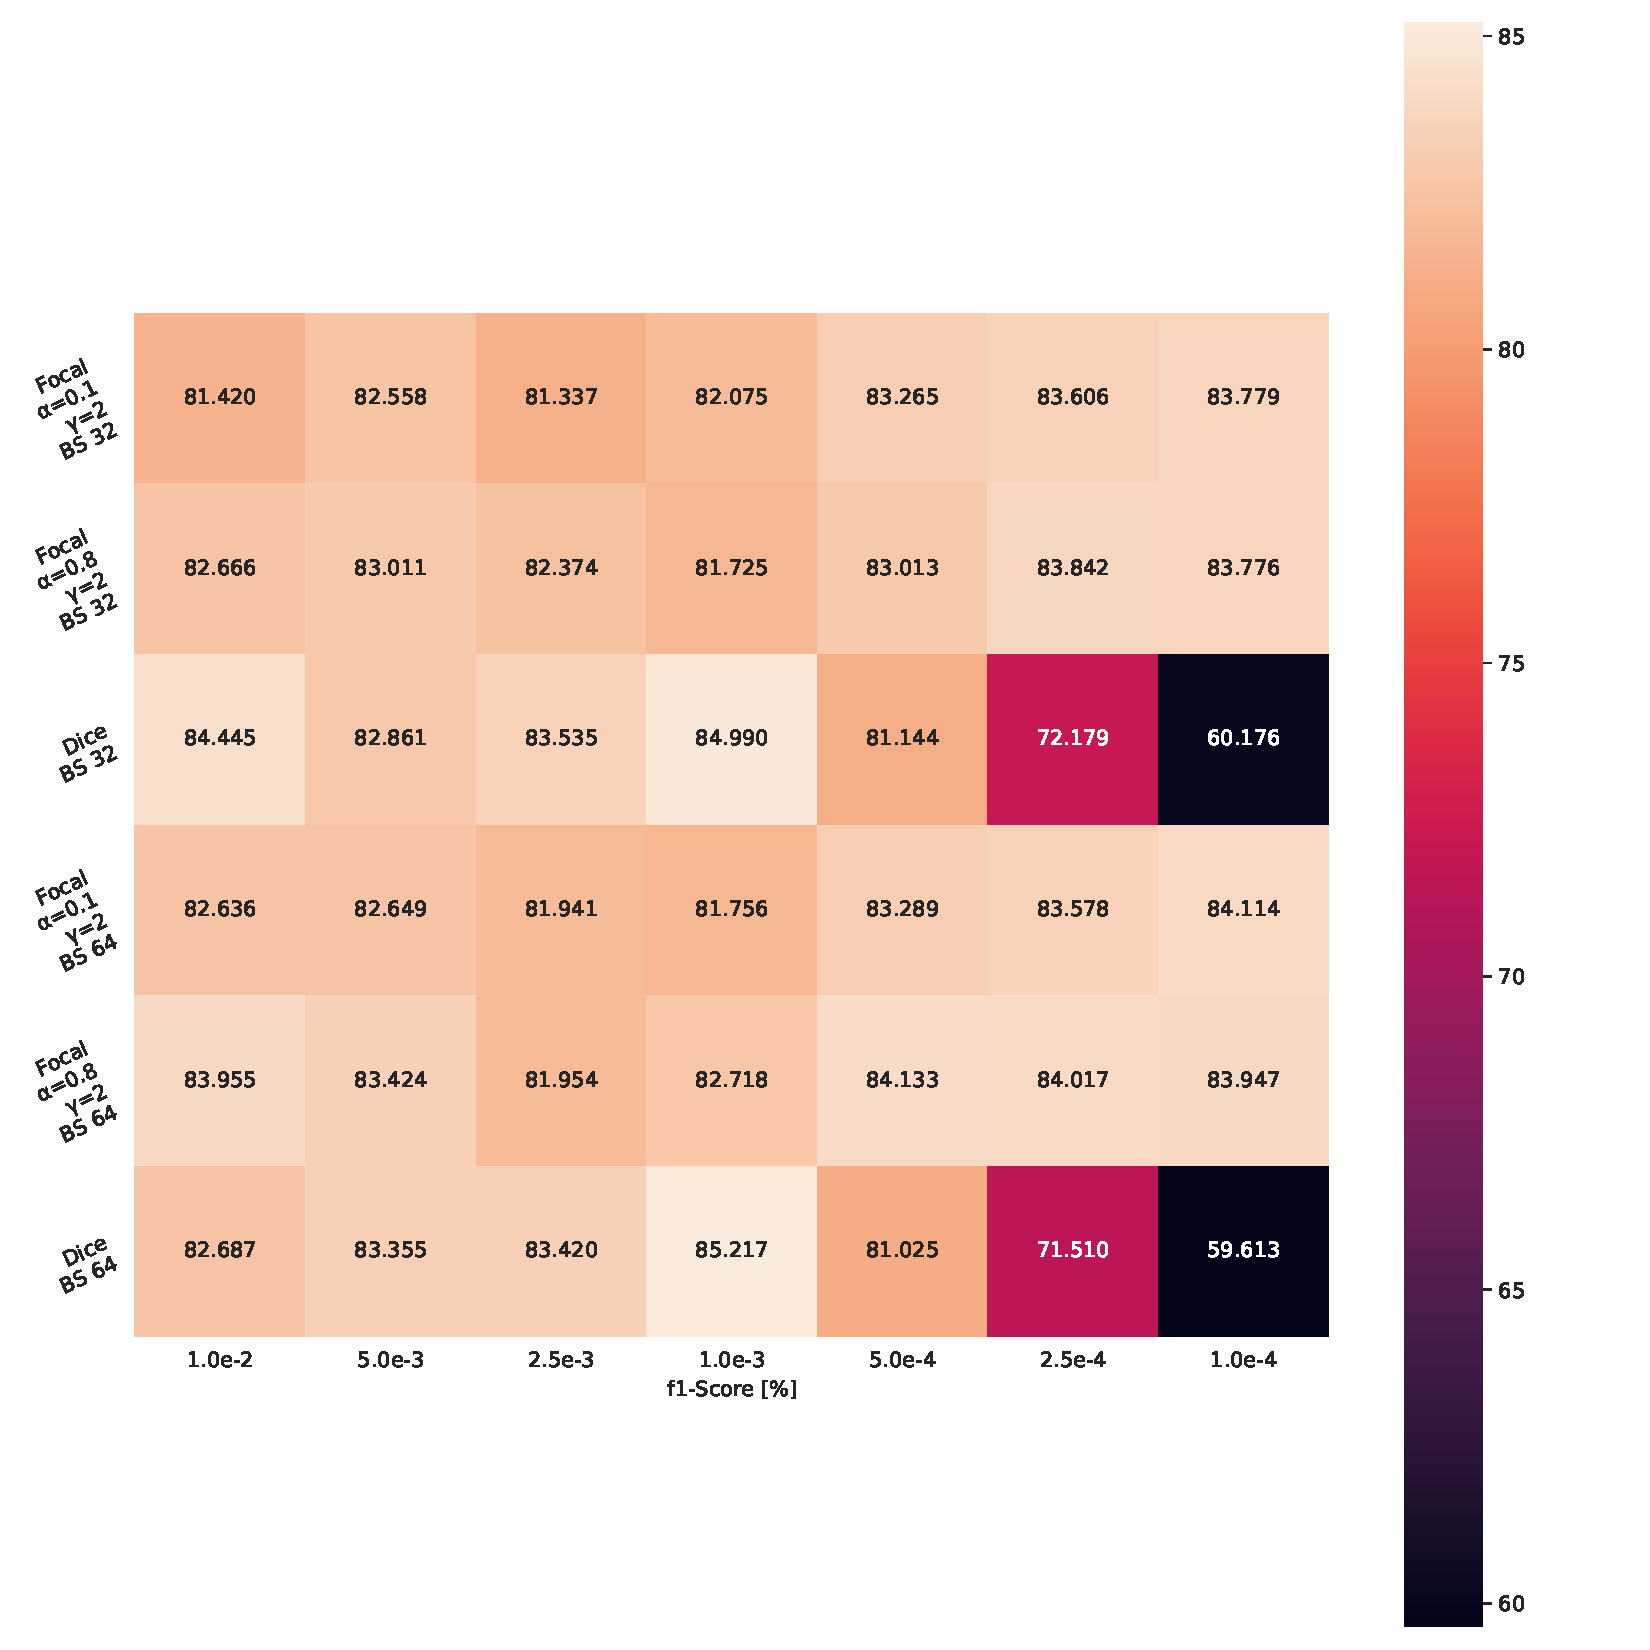
\includegraphics[width=\columnwidth]{imgs/munet_grid_heat_F1_C.pdf}
    \caption{F1-Score results of the \ac{MUnet} grid search experiment shown validation data, for checkered images only. Results are shown combined for the loss and batch size against the learning rate.}
    \label{fig:munet_f1c_heat}
\end{center}
\end{figure}

\begin{figure}[H]
\begin{center}
    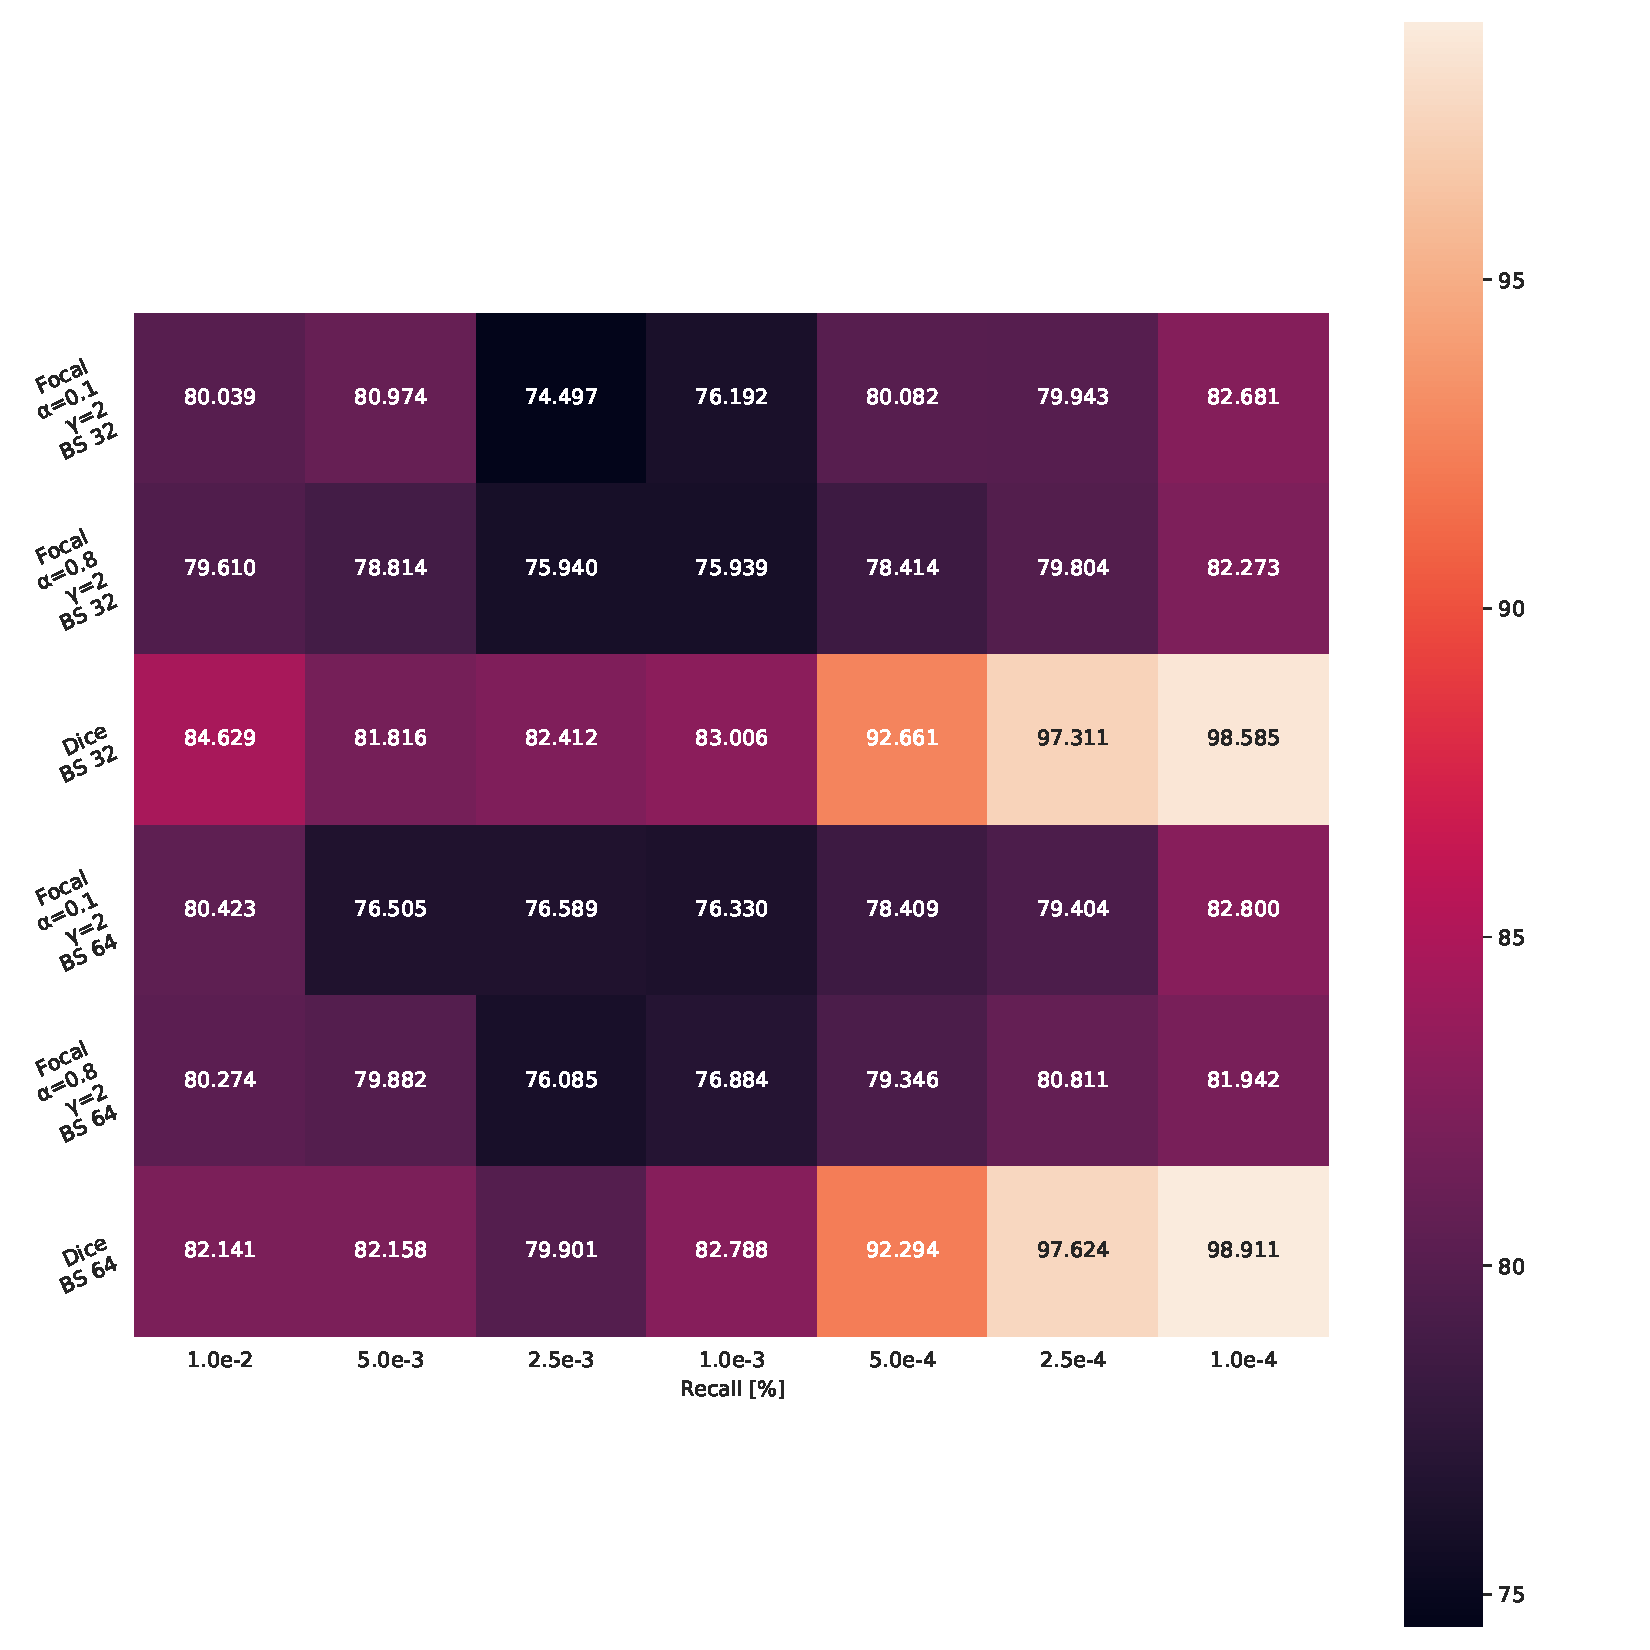
\includegraphics[width=\columnwidth]{imgs/munet_grid_heat_R_C.pdf}
    \caption{Recall results of the \ac{MUnet} grid search experiment shown validation data, for checkered images only. Results are shown combined for the loss and batch size against the learning rate.}
    \label{fig:munet_rc_heat}
\end{center}
\end{figure}

\begin{figure}[H]
\begin{center}
    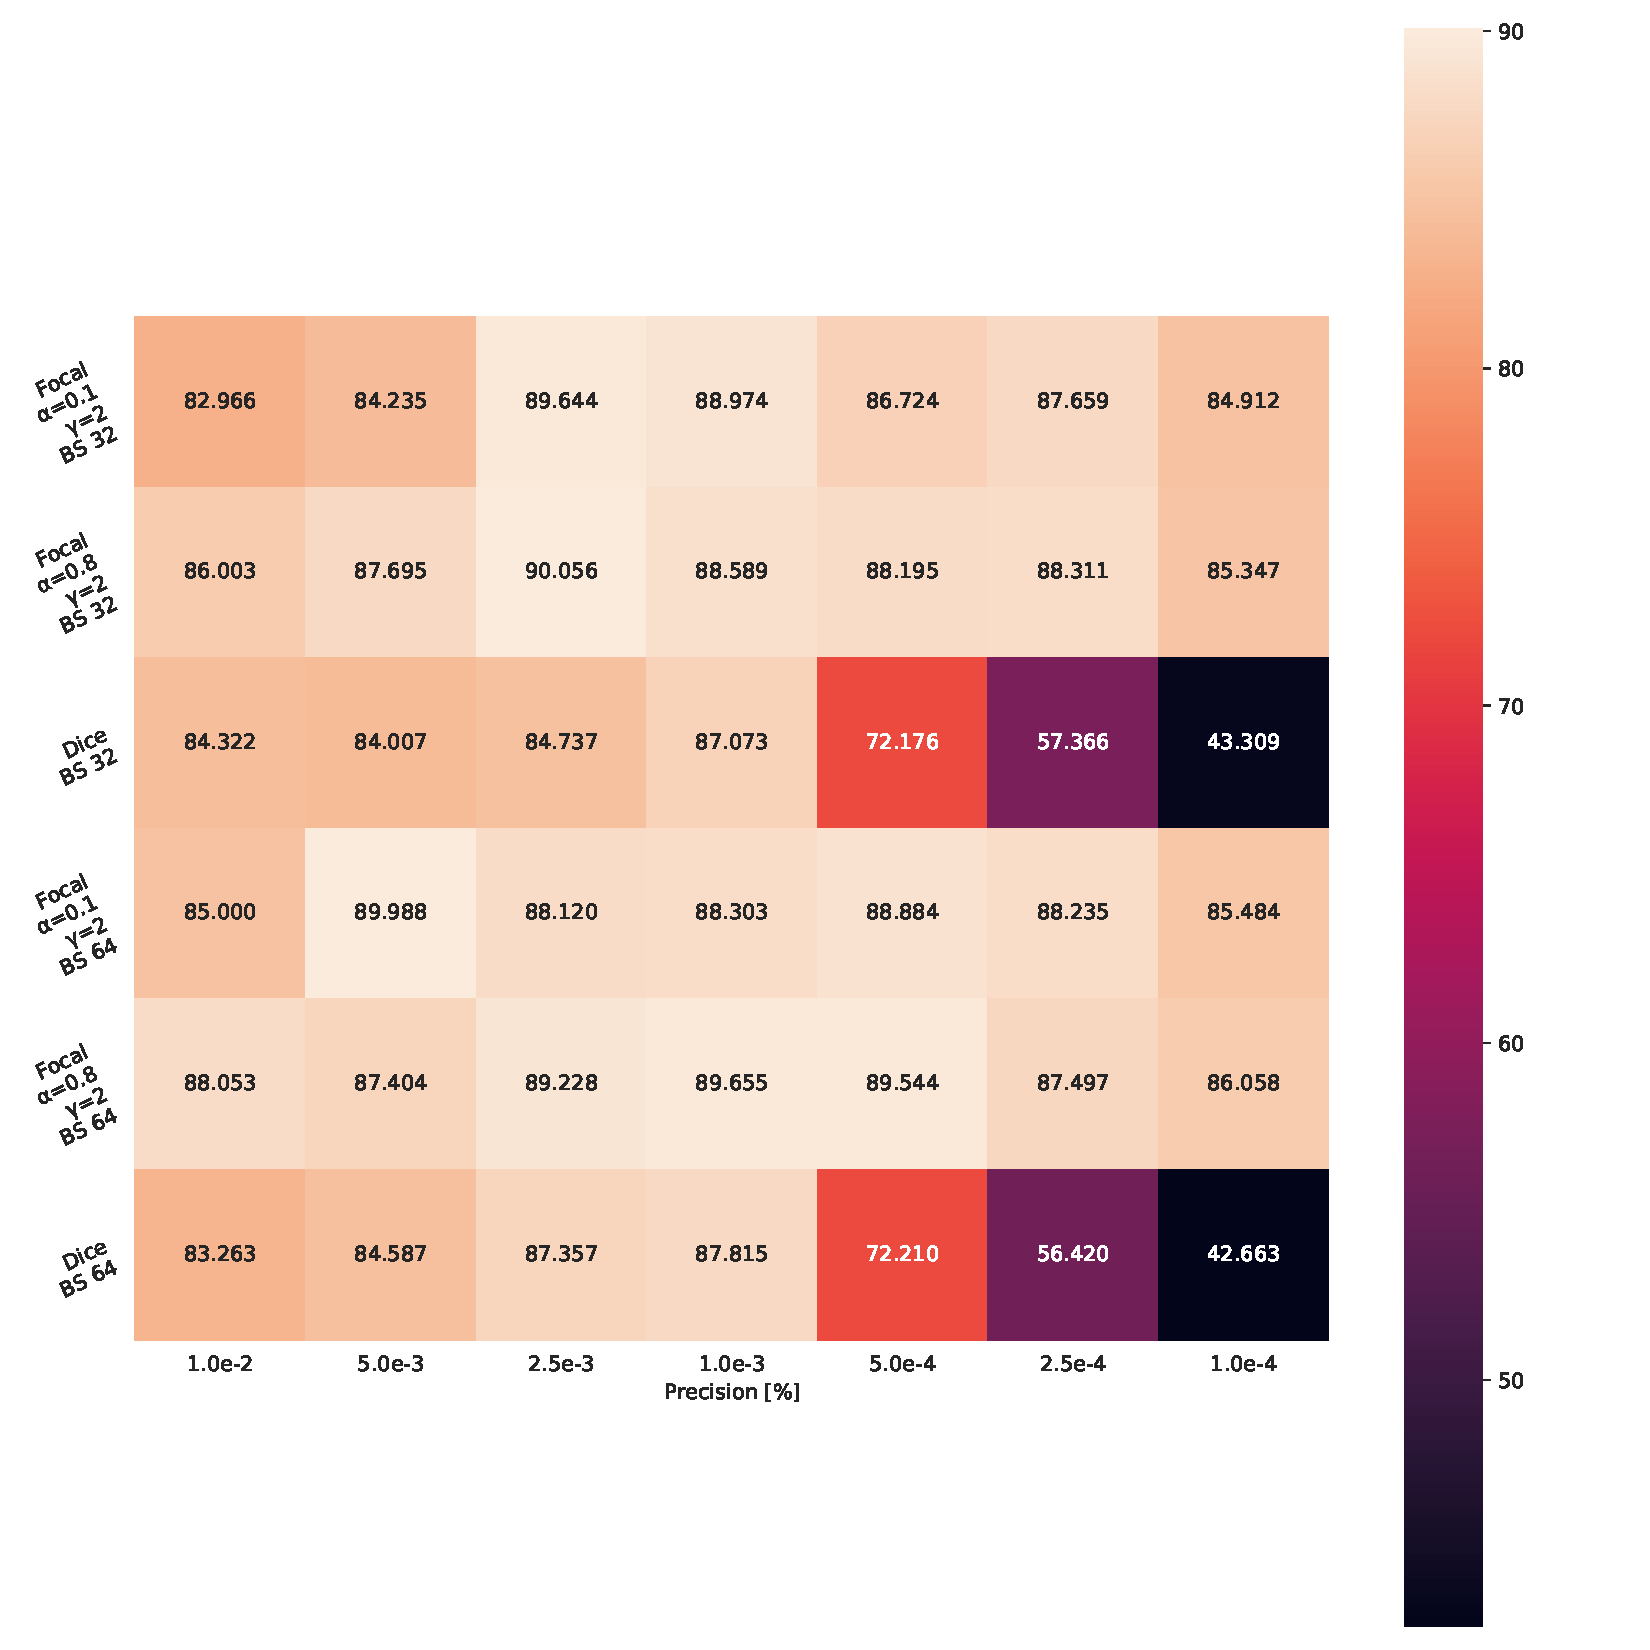
\includegraphics[width=\columnwidth]{imgs/munet_grid_heat_P_C.pdf}
    \caption{Precision results of the \ac{MUnet} grid search experiment shown validation data, for checkered images only. Results are shown combined for the loss and batch size against the learning rate.}
    \label{fig:munet_pc_heat}
\end{center}
\end{figure}

\begin{table}[H]
\footnotesize
\begin{center}
\begin{tabular}{|l|l|l|l|l|l|}

\hline
\textbf{Batch Size} & \textbf{Loss} & \textbf{Learning Rate} & \textbf{Dataset Type} &\textbf{Metric} & \textbf{Metric Value} \\
\hline
32  & Focal $\gamma = 2$, $\alpha = 0.1$  & $1.0e^{-2}$& Full      & F1        & 84.3573  \\
\hline
32  & Focal $\gamma = 2$, $\alpha = 0.1$  & $1.0e^{-4}$& Full      & Recall    & 86.273   \\
\hline
32  & Focal $\gamma = 2$, $\alpha = 0.1$  & $2.5e^{-3}$& Full      & Precision & 86.6923  \\
\hline
32  & Focal $\gamma = 2$, $\alpha = 0.1$  & $1.0e^{-4}$& Checkered & F1        & 83.779   \\
\hline
32  & Focal $\gamma = 2$, $\alpha = 0.1$  & $1.0e^{-4}$& Checkered & Recall    & 82.6813  \\
\hline
32  & Focal $\gamma = 2$, $\alpha = 0.1$  & $2.5e^{-3}$& Checkered & Precision & 89.6437  \\
\hline
32  & Focal $\gamma = 2$, $\alpha = 0.8$  & $5.0e^{-3}$& Full      & F1        & 84.624   \\
\hline
32  & Focal $\gamma = 2$, $\alpha = 0.8$  & $1.0e^{-4}$& Full      & Recall    & 85.8127  \\
\hline
32  & Focal $\gamma = 2$, $\alpha = 0.8$  & $2.5e^{-3}$& Full      & Precision & 85.9127  \\
\hline
32  & Focal $\gamma = 2$, $\alpha = 0.8$  & $2.5e^{-4}$& Checkered & F1        & 83.8423  \\
\hline
32  & Focal $\gamma = 2$, $\alpha = 0.8$  & $1.0e^{-4}$& Checkered & Recall    & 82.273   \\
\hline
32  & Focal $\gamma = 2$, $\alpha = 0.8$  & $2.5e^{-3}$& Checkered & Precision & 90.0563  \\
\hline
32  & Dice                                & $1.0e^{-2}$& Full      & F1            & 85.449   \\
\hline
32  & Dice                                & $1.0e^{-4}$& Full      & Recall        & 99.1407  \\
\hline
32  & Dice                                & $5.0e^{-3}$& Full      & Precision     & 83.2367  \\
\hline
32  & Dice                                & $1.0e^{-3}$& Checkered & F1            & 84.9903  \\
\hline
32  & Dice                                & $1.0e^{-4}$& Checkered & Recall        & 98.5847  \\
\hline
32  & Dice                                & $1.0e^{-3}$& Checkered & Precision     & 87.0733  \\
\hline
64  & Focal $\gamma = 2$, $\alpha = 0.1$  & $1.0e^{-2}$& Full      & F1        & 84.523   \\
\hline
64  & Focal $\gamma = 2$, $\alpha = 0.1$  & $1.0e^{-4}$& Full      & Recall    & 86.31    \\
\hline
64  & Focal $\gamma = 2$, $\alpha = 0.1$  & $2.5e^{-3}$& Full      & Precision & 85.599   \\
\hline
64  & Focal $\gamma = 2$, $\alpha = 0.1$  & $1.0e^{-4}$& Checkered & F1        & 84.114   \\
\hline
64  & Focal $\gamma = 2$, $\alpha = 0.1$  & $1.0e^{-4}$& Checkered & Recall    & 82.8     \\
\hline
64  & Focal $\gamma = 2$, $\alpha = 0.1$  & $5.0e^{-3}$& Checkered & Precision & 89.9877  \\
\hline
64  & Focal $\gamma = 2$, $\alpha = 0.8$  & $1.0e^{-2}$& Full      & F1        & 84.879   \\
\hline
64  & Focal $\gamma = 2$, $\alpha = 0.8$  & $1.0e^{-4}$& Full      & Recall    & 85.5173  \\
\hline
64  & Focal $\gamma = 2$, $\alpha = 0.8$  & $1.0e^{-2}$& Full      & Precision & 84.8933  \\
\hline
64  & Focal $\gamma = 2$, $\alpha = 0.8$  & $5.0e^{-4}$& Checkered & F1        & 84.133   \\
\hline
64  & Focal $\gamma = 2$, $\alpha = 0.8$  & $1.0e^{-4}$& Checkered & Recall    & 81.942   \\
\hline
64  & Focal $\gamma = 2$, $\alpha = 0.8$  & $1.0e^{-3}$& Checkered & Precision & 89.655   \\
\hline
64  & Dice                                & $5.0e^{-3}$& Full      & F1            & 84.52    \\
\hline
64  & Dice                                & $1.0e^{-4}$& Full      & Recall        & 99.279   \\
\hline
64  & Dice                                & $2.5e^{-3}$& Full      & Precision     & 84.5423  \\
\hline
64  & Dice                                & $1.0e^{-3}$& Checkered & F1            & 85.2167  \\
\hline
64  & Dice                                & $1.0e^{-4}$& Checkered & Recall        & 98.911   \\
\hline
64  & Dice                                & $1.0e^{-3}$& Checkered & Precision     & 87.815   \\
\hline

\end{tabular}
\caption{The selected \ac{MUnet} folds (combination of batch size and loss) from the grid search experiment. From each fold the best performing metrics were selected, based on the full validation set and the validation set with checkered backgrounds only. The metric values indicate the mean score of that particular fold. From each fold then the best performing training run has been selected as a network for further testing. Overall 36 folds have been selected. Some combinations appeared more then once, hence overall 26 networks have been in the end selected.}
\label{tab:munet_selected_nets}
\end{center}
\end{table}
